% !TEX program = xelatex
% Example: PGFPlots data from file
\documentclass[11pt, a4paper]{article}
\usepackage{pgfplots}
\pgfplotsset{compat=1.18}

\begin{document}

\section*{رسمُ البياناتِ من ملف}

% بياناتٌ مُضمّنةٌ في المستند
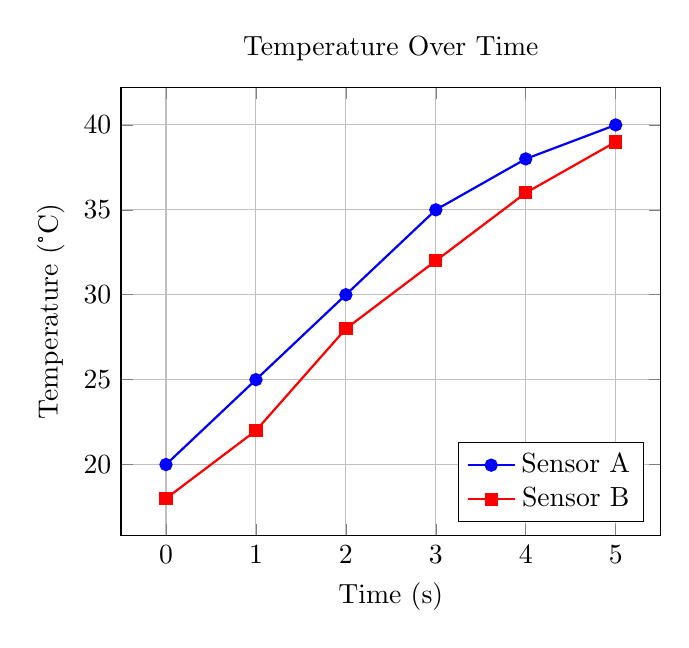
\begin{tikzpicture}
\begin{axis}[
  xlabel={Time (s)},
  ylabel={Temperature (\textdegree C)},
  title={Temperature Over Time},
  grid=major,
  legend pos=south east,
  mark size=2pt
]
  \addplot[blue, thick, mark=*] table {
    x y
    0 20
    1 25
    2 30
    3 35
    4 38
    5 40
  };
  \addlegendentry{Sensor A}

  \addplot[red, thick, mark=square*] table {
    x y
    0 18
    1 22
    2 28
    3 32
    4 36
    5 39
  };
  \addlegendentry{Sensor B}
\end{axis}
\end{tikzpicture}

\end{document}
